\subsection*{1}
    %Build a noninverting amplifier circuit as shown below. Use R1 = 100  and R2 = 10 k 
    %so that the amplifier gain is about 100.

    A non inverting amplifier circuit as shown in figure X below. The amplifier gain should be about 100 so resistances R$_1$ = 100 $\Omega$ and R$_2$ = 10 k$\Omega$ were used.

    \begin{figure}[h!]
        \centering
        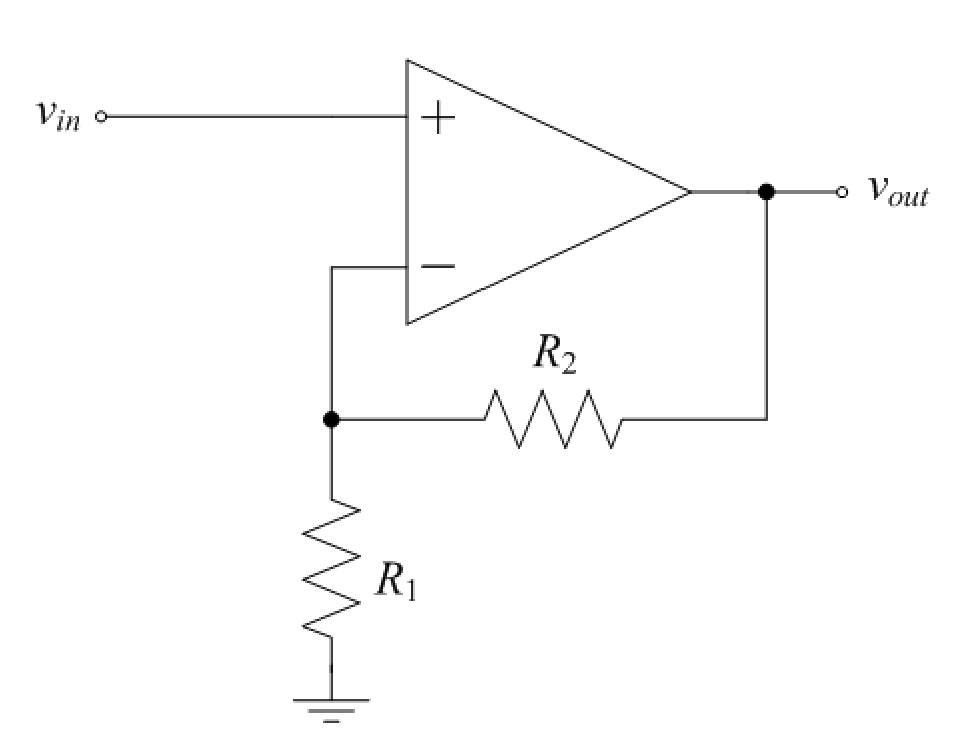
\includegraphics[width=6cm]{task2_1.png}
        \captionof{figure}{}
    \end{figure}

\subsection*{2}
    %Using  a  Bode  Analyzer  measure  the  AC  characteristics  of  the  circuit in  the  frequency
    %range 100 Hz to 50 kHz. Use 10 steps per decade and input signal amplitude of 20 mV.
    %Find the gain-bandwidth product (GBW) of the operational amplifier and compare it to
    %the nominal value (1 MHz). 

    A Bode Analyzer was used to measure the AC characteristics of the circuit in the frequency range 100 Hz to 50kHz using 10 steps per decade and an input signal amplitude of 20 mV.\\

    %FIGURE OF THE AC ANALYSIS
    %gainið sem kemur upp í kringum 3dB freq er vegna noise í mælingum
    \begin{figure}[h!]
        \centering
        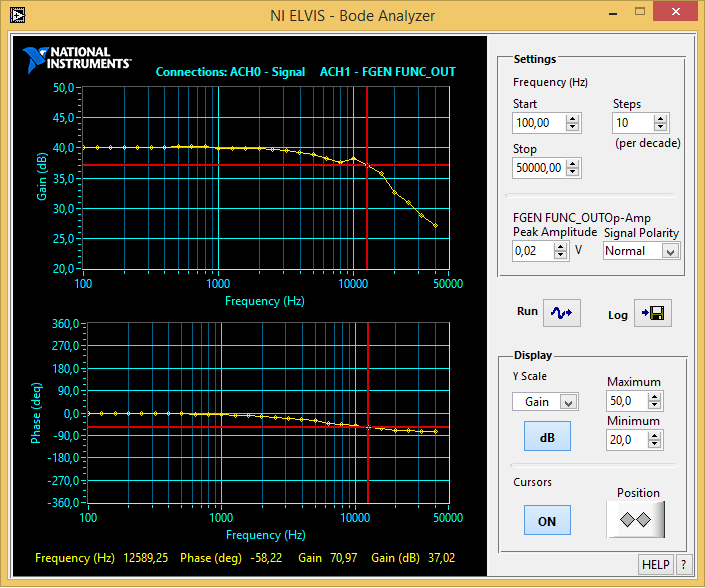
\includegraphics[width=6cm]{task2_2_cursor.png}
        \captionof{figure}{}
    \end{figure}

    The gain-bandwidth product (GBW) of the operational amplifier was found using the values read from the oscilloscope seen in figure X above.

    $$f_{3dB} = f_{H} = 12.6 kHz$$

    $$\text{gain-bandwidth product} = f_{3dB} \cdot (\frac{R_2}{R_1} + 1) = 12.6\text{ kHz} \cdot (\frac{9.96\ k \Omega}{100.2\ \Omega} + 1) = 1.26 \text{ MHz}$$

    The nominal gain-bandwidth product of the LM741 operational amplifier is 1 MHz. The measured gain is similar compared to the nomial gain.

    \begin{table}[htbp]
     \centering
     \caption{Comparison between theoretical and measured value}
       \begin{tabular}{c|c}
        \multicolumn{2}{c}{Gain-Bandwidth Product}\\
        \hline
        Actual value [MHz] & Theoretical value [MHz] \\
       \hline
        1.26          & 1 \\
       \end{tabular}%
     \label{tab:addlabel}%
   \end{table}%

\subsection*{3}
    %Build a voltage follower circuit as shown below:

    A voltage follower circuit was built as seen in figure X below.\\
    
    \begin{figure}[h!]
        \centering
        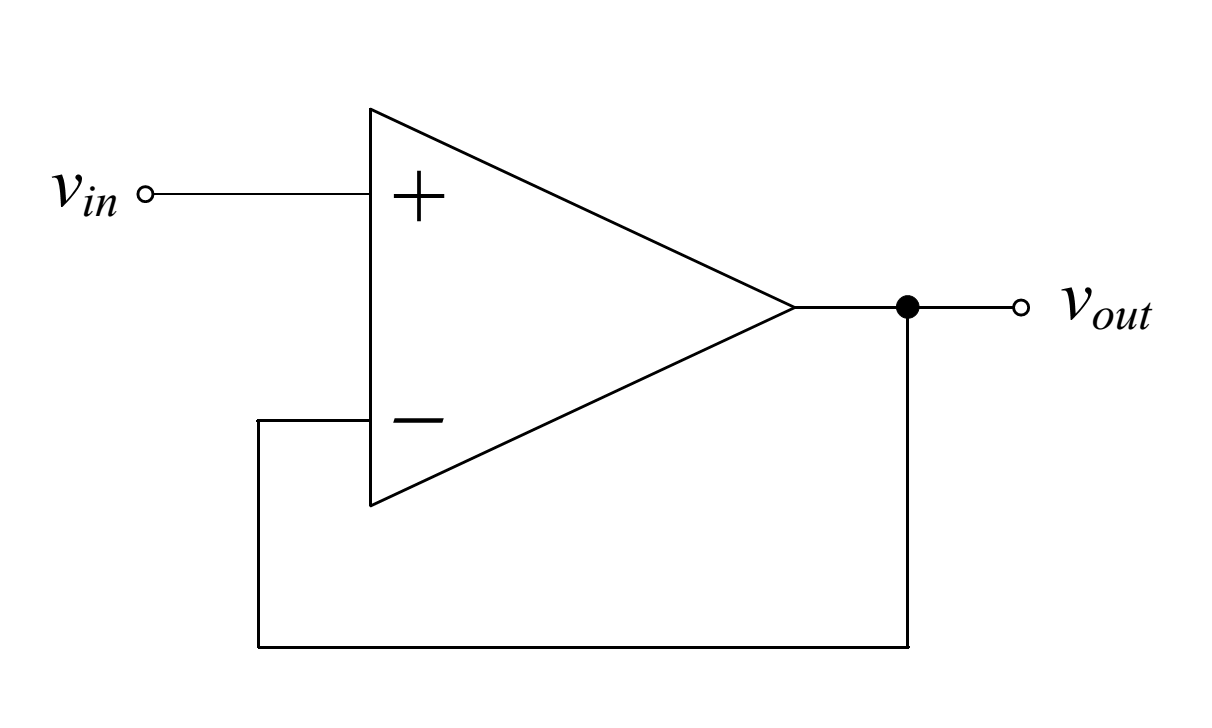
\includegraphics[width=6cm]{task2_3.png}
        \captionof{figure}{}
    \end{figure}


\subsection*{4}
    %Apply  a  rectangular  waveform  (amplitude  around  2.5 V)  to  the  input  of  the  circuit  and
    %observe both the input and the output signal using the oscilloscope. Determine the slew- 
    %rate (SR) of the operational amplifier and compare it to the nominal value (0.5 V/µs).